\documentclass[aspectratio=169,11pt]{beamer}
\usepackage{assets/ide-beamer}
\title[Ide \& Talamàs: capacidad y autonomía]{Artificial Intelligence\\in the Knowledge Economy}
\subtitle{Una auditoría de la lectura distributiva}
\author{Belén Vásquez}
\institute{Modelamiento Económico con IA}
\date{Septiembre de 2026}
\newcommand{\aAI}{z_{\mathrm{AI}}}
\begin{document}

\begin{frame}[plain]
\titlepage
\vspace{-1cm}
\begin{center}\small\href{\RepoURL}{\texttt{\RepoURL}}\end{center}
\sourcefoot{\paperref, p. 1; JPE 133(12), 3762--3800. Fuente trabajada: v11, 35 pp.}
\end{frame}

\begin{frame}{El problema de la firma}
\begin{columns}[T,onlytextwidth]
\column{.51\textwidth}
Un worker intenta un problema $x\sim U[0,1]$; consulta si $x>z$.
\[
 hn(z)(1-z)=1\quad\Rightarrow\quad n(z)=\frac1{h(1-z)}.
\]
Si el solver sabe $s\ge z$, el producto esperado del equipo es $n(z)s$.
\column{.46\textwidth}
\[
\max_{z,s}\ n(z)[s-w(z)]-w(s).
\]
La firma elige conocimientos, ocupaciones y tecnología. Competencia: beneficios cero.
\[
\int_Yh(1-z)dG(z)=\int_{m(Y)}dG(s).
\]
\end{columns}
\medskip
\begin{keybox}El tiempo del experto es escaso. El emparejamiento $m'(z)>0$ es un resultado de equilibrio.\end{keybox}
\sourcefoot{\paperref, §3.1, pp. 10--13; Prop. 1 y FOC, pp. 16--18.}
\end{frame}

\begin{frame}{Dominio de las proposiciones}
\small
\begin{itemize}
\item Masa humana y tiempo individual: 1. $z\in[0,1]$ observable y fijo; $g$ continua y positiva. Problemas independientes, éxito si $z>x$.
\item Firmas competitivas, sin costo fijo, agentes neutrales al riesgo, máximo dos capas; consultas cuestan $h\in(0,1)$ aun si fallan.
\item Restricción mantenida: $\alert{h<h_0(G)}$; no hay independientes humanos antes de IA.
\item IA común, sustituto perfecto: $a=\aAI\in[0,1)$; una unidad de cómputo por agente. Oportunidades abundantes.
\item Mismo cómputo exógeno y abundante al comparar autonomías:
\[
\int_0^a h(1-z)dG(z)+\frac{1-G(a)}{h(1-a)}<\mu
\quad\text{es suficiente.}
\]
\end{itemize}
\textbf{Dos dimensiones:} capacidad $a$; autonomía para producir además de asesorar.
\sourcefoot{\paperref, §3.1 pp. 9--13, nota 14; restricción p. 18; §6 p. 26.}
\end{frame}

\begin{frame}{Proposición 5: el umbral es de capacidad}
Bajo el dominio anterior, con autonomía:
\[
B=\{z\le a:w^A(z)>w(z)\}=[0,z_b),\qquad
T=\{z\ge a:w^A(z)>w(z)\}=(z_t,1].
\]
\begin{block}{Resultado completo}
Existe $\bar a\in\operatorname{int}W$ tal que
\[
 B\ne\varnothing\iff a>\bar a.
\]
Para todo $a\in[0,1)$, $T\ne\varnothing$.
\end{block}
\begin{keybox}Hay ganadores arriba; ganar abajo exige capacidad suficiente. No significa que todos los workers pierdan ni que todos ganen.\end{keybox}
La garantía superior usa $h<h_0$ y excluye $a=1$.
\sourcefoot{\paperref, Prop. 5, p. 24; forma de B y T, p. 24; límites, p. 25, nota 19.}
\end{frame}

\begin{frame}{Proposición 6: adopción y eficiencia restringida}
\small
Con IA solo co-pilot y el mismo dominio:
\begin{itemize}
\item Equilibrio único, eficiente dentro de su conjunto factible; maximiza ingreso laboral y $r^N=0$.
\item Si $a\le w(0)$: IA no se usa; salarios y ocupaciones son los pre-IA.
\item Si $a>w(0)$: solo la base usa IA como solver,
\[
W_a^N\preceq W_p^N\cup I^N\cup S_p^N,
\]
con todos esos conjuntos no vacíos salvo posiblemente $I^N$.
\end{itemize}
\begin{block}{Derivación del umbral de adopción}
\[
n(z)[a-w^N(z)]-0=0\ \Rightarrow\ w^N(z)=a.
\]
Si $a\le w(0)$, no mejora ninguna oferta previa, pues $w(z)$ es creciente. Si $a>w(0)$, es rentable entrar a salarios previos de la base.
\end{block}
\sourcefoot{\paperref, Prop. 6, pp. 26--27; reconstrucción propia de beneficio cero.}
\end{frame}

\begin{frame}{Proposición 6: las cuatro comparaciones}
\small
\begin{enumerate}
\item Producto: $Y^A>Y^N$.
\item Existe $z\in(0,1]$ con $w^N(z)\le w(z)$; estricta si $a>w(0)$.
\item Existe $\epsilon>0$ tal que, para $z\in[0,\epsilon)$:
\[
 w^N(z)\ge\max\{w(z),w^A(z)\};
\]
la desigualdad es estricta si $a>w(0)$.
\item Existe $\epsilon>0$ tal que, para $z\in(1-\epsilon,1]$:
\[
 w^N(z)\le w^A(z);
\]
la desigualdad es estricta si $z\ne1$.
\end{enumerate}
\begin{keybox}``Los menos conocedores ganan'' necesita distinguir ganancia débil, ganancia estricta y adopción.\end{keybox}
\sourcefoot{\paperref, Prop. 6, p. 27. Supuestos de la diapositiva 3.}
\end{frame}

\begin{frame}{Comparar umbrales requiere identificar al solver}
\small
Con autonomía, $r^A=a$ y $w^A(a)=a$. Sea $s_A$ el solver marginal que atiende a la base, humano o IA:
\[
w^A(0)=(1-h)s_A,\qquad s_A(\bar a)=\frac{w(0)}{1-h}.
\]
En el cruce, por crecimiento salarial estricto:
\[
 w(0)=w^A(0;\bar a)<w^A(\bar a;\bar a)=\bar a.
\]
La oferta worker--IA garantiza $w^A(0)\ge(1-h)a$. Por tanto:
\begin{keybox}
\[
\boxed{w(0)<\bar a\le\frac{w(0)}{1-h}}.
\]
\end{keybox}
La cota superior es identidad solo si la base usa IA al cruzar. La prueba general de cruce único se toma de Prop. 5.
\sourcefoot{Derivación propia usando Prop. 2, pp. 19--21, y Prop. 5, p. 24.}
\end{frame}

\begin{frame}{Especialización uniforme: umbrales cuantificados}
\small
Para $G(z)=z$, $h_0=3/4$. Sea $c$ el límite pre-IA y $C=w(c)$.
\[
c+h(c-c^2/2)=1,\quad
C=\frac{1-hc(1-c)}{1+h(1-c)},\quad w(0)=c-hC.
\]
\begin{center}
\begin{tabular}{lrr}
\toprule
$h$ & $w(0)$ & $\bar a$ \\
\midrule
$0.5$ & $0.357044$ & $0.714087$ \\
$0.7$ & $0.197966$ & $0.609745$ \\
\bottomrule
\end{tabular}
\end{center}
Con $h=.7$, $\bar a<w(0)/(1-h)=.659885$: en el cruce asesora un humano.
\begin{keybox}La capacidad para ayudar a la base con autonomía depende también de organización, $h$ y distribución $G$.\end{keybox}
\sourcefoot{Derivación propia, extensions.md §4; base: Prop. 1, pp. 16--18; Fig. 3, p. 17.}
\end{frame}

\begin{frame}{Dos tipos: derivación propia hasta el umbral}
\small
$z_L=0$, $z_H=H<1$, $\mu_L=\mu_H=1/2$. Sobran humanos altos para producir solos: $w_H=H$, $w_L=(1-h)H$.
\[
 a<H:\quad v_H=\max\{H,(H-a)/[h(1-a)]\},
\]
\[
 w_L^A=\max\{0,H-hv_H,(1-h)a\}.
\]
Como $v_H\ge H$, para $a\le H$ ninguna oferta supera $(1-h)H$. Para $a>H$, $w_L^A=(1-h)a$.
\[
w_L^N=\max\{(1-h)H,a\}.
\]
\begin{keybox}
\[
w_L^A>w_L\iff a>H;\qquad w_L^N>w_L\iff a>(1-h)H.
\]
\end{keybox}
Esta economía tiene masas e independientes pre-IA: no prueba la Prop. 5 del continuo.
\sourcefoot{Derivación propia, hand/README.md; tecnologías de §3.1, pp. 10--13.}
\end{frame}

\begin{frame}{Un equilibrio discreto con conflicto estricto}
\small
$H=.8$, $h=.5$, $a=.6$, $\mu=10$, masas humanas $(.5,.5)$.
\begin{center}
\begin{tabular}{lrrr}
\toprule
 & Sin IA & Autónoma & Solo co-pilot\\
\midrule
Salario bajo & .4 & .3 & .6\\
Salario alto & .8 & 1 & .8\\
Producto total & .6 & 6.65 & .7\\
\bottomrule
\end{tabular}
\end{center}
A: .5 workers humanos consultan a .25 IA; .5 expertos humanos ayudan a 2.5 workers IA; 7.25 IA producen solos.
\[
Y^A=.5(.6)+2.5(.8)+7.25(.6)=6.65.
\]
\begin{keybox}El cómputo es el mismo en A y N; en N queda ocioso. El tamaño del aumento no es una estimación de PIB ni una calibración.\end{keybox}
\sourcefoot{sim.py y extensions.md §6, ejemplo propio; identidades de producto: §3.1, p. 13.}
\end{frame}

\begin{frame}{Salarios y región de conflicto}
\centering
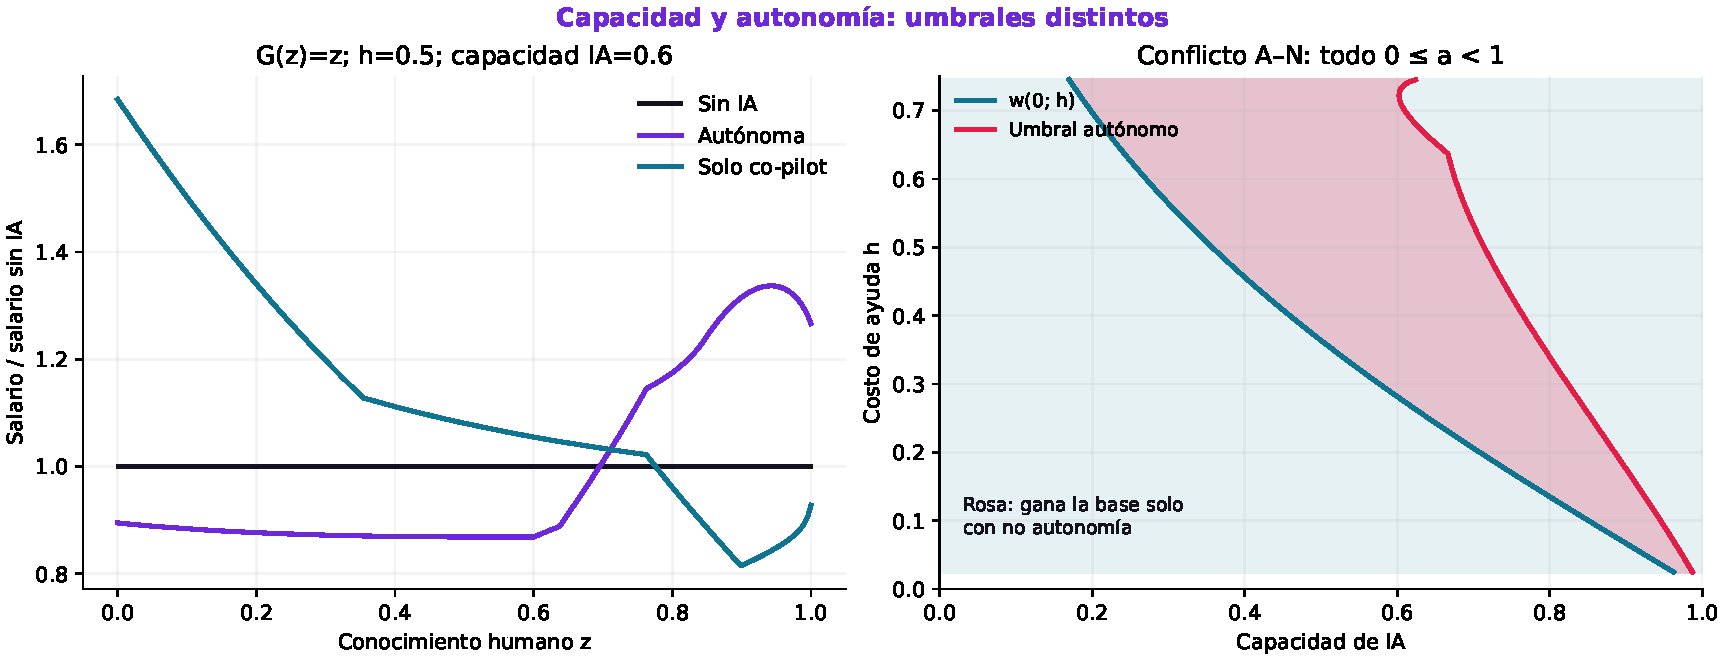
\includegraphics[width=.97\linewidth,height=.66\textheight,keepaspectratio]{extra/figures/bottom-winners-threshold.pdf}
\par\small Conflicto estricto A--N: todo $0\le a<1$. Franja rosa: $w(0;h)<a\le\bar a(h)$; solo N beneficia estrictamente a la base frente a no IA.
\sourcefoot{sim.py: LP, malla uniforme 241 nodos; frontera analítica propia. Prop. 6, p. 27.}
\end{frame}

\begin{frame}{Qué cambia en los extremos}
\small
\begin{tabular}{p{.19\linewidth}p{.73\linewidth}}
\toprule
Extremo & Límite de la interpretación\\
\midrule
$a=0$ & N no se adopta; A puede ser worker que consulta todo. Capacidad cero no elimina su tiempo productivo.\\[.8em]
$a\to1^-$ & Ganadores arriba para cada $a<1$; no asegura un intervalo ganador uniforme. $a=1$ está excluido.\\[.8em]
$h\to0^+$ & $n(z)$ diverge; puede fallar abundancia con cómputo fijo. En la especialización uniforme los umbrales tienden a 1.\\[.8em]
$h\to1^-$ & Antes se cruza $h_0(G)<1$. La garantía de ganadores superiores no se extiende automáticamente.\\
\bottomrule
\end{tabular}
\sourcefoot{Prop. 5, pp. 24--25, nota 19; §3.1 pp. 10--13, notas 11 y 14; límite uniforme propio.}
\end{frame}

\begin{frame}{El supuesto de sustitución perfecta hace trabajo}
\begin{itemize}
\item Sostiene $w^A(a)=a$: el humano directamente sustituible pierde su renta organizativa.
\item Conocimientos anidados: una IA no resuelve excepciones que otra IA idéntica desconoce. Una jerarquía IA--IA no añade capacidad.
\item No hay verificación costosa, aprendizaje ni error estocástico adicional; el modelo sí comparte fallos frente a dificultades mayores que $a$.
\end{itemize}
\begin{keybox}Extensión parcial propia: con costo de revisión $k$ por worker, la oferta co-pilot pasa a $a-k$; la entrada en la base exige $a>w(0)+k$. No es aún un equilibrio general resuelto.\end{keybox}
\sourcefoot{§3.1, pp. 9--13; Prop. 2, pp. 19--20. Extensión y crítica propias, extensions.md §8.}
\end{frame}

\begin{frame}[fragile]{Lean: nueve lemas probados; equilibrio pendiente}
\footnotesize
\textbf{1. Ecuaciones y traducción condicional.}
\[
n(z)=\frac{1}{h(1-z)},\quad n(z)(a-w)-r=0,\quad r=0
\ \Longrightarrow\ w>w_0\iff a>w_0.
\]
\textbf{2. Enunciado y prueba reales de MainTheorems.lean.}
\begin{lstlisting}[basicstyle=\ttfamily\fontsize{7}{8}\selectfont,escapeinside={(*@}{@*)}]
theorem nonautonomous_bottom_improvement_iff
    {h z aiKnowledge workerWage preAIWage : (*@$\mathbb{R}$@*)}
    (h_pos : 0 < h)
    (z_lt_one : z < 1)
    (zeroProfit : topAutomatedProfit h z aiKnowledge workerWage 0 = 0) :
    workerWage > preAIWage (*@$\leftrightarrow$@*) aiKnowledge > preAIWage := by
  rw [nonautonomous_workerWage_eq_aiKnowledge h_pos z_lt_one zeroProfit]
\end{lstlisting}
\textbf{3. Mi interpretación.} Reales, $h>0$, $z<1$ y beneficio cero: Lean sustituye $w=a$. \alert{No prueba que el trabajador use IA en equilibrio.} Las Props. 5 y 6 siguen pendientes; el umbral autónomo probado es condicional al solver IA.

\medskip
\textbf{4. Verificación real.} Python 3.12.14; \texttt{check --fast}: exit 0. Nueve lemas sin \texttt{sorryAx}; build completo: seis advertencias \texttt{sorry} en las proposiciones. \alert{Check rápido exitoso no significa paper demostrado.}
\sourcefoot{Tecnología: §3.1, pp. 9--12; renta cero: Prop. 6, p. 27. Deducción condicional propia. lean/CHECK\_OUTPUT.txt, BUILD\_OUTPUT.txt y AXIOM\_OUTPUT.txt.}
\end{frame}

\begin{frame}{Evidencia manuscrita: qué demuestra la hoja}
\begin{columns}[T,onlytextwidth]
\column{.51\textwidth}
\small
\textbf{Foto real aportada por la estudiante.}
\[
n(z)=\frac{1}{h(1-z)},\quad w=a-rh(1-z).
\]
Con $r=0$, un worker asignado a IA recibe $w=a$: su ganancia exige $a>w(0)$.

\medskip
\textbf{Alcance.} La hoja enuncia el umbral autónomo. \alert{No desarrolla el equilibrio discreto de dos tipos ni deriva su umbral.} Ese desarrollo está tipeado en \texttt{hand/README.md} y \texttt{extensions.md}.

\medskip
\textbf{Veredicto.} La capacidad cruza los umbrales; la autonomía también cambia los usos y el costo de oportunidad. No se reduce a mover un número.
\column{.46\textwidth}
\centering
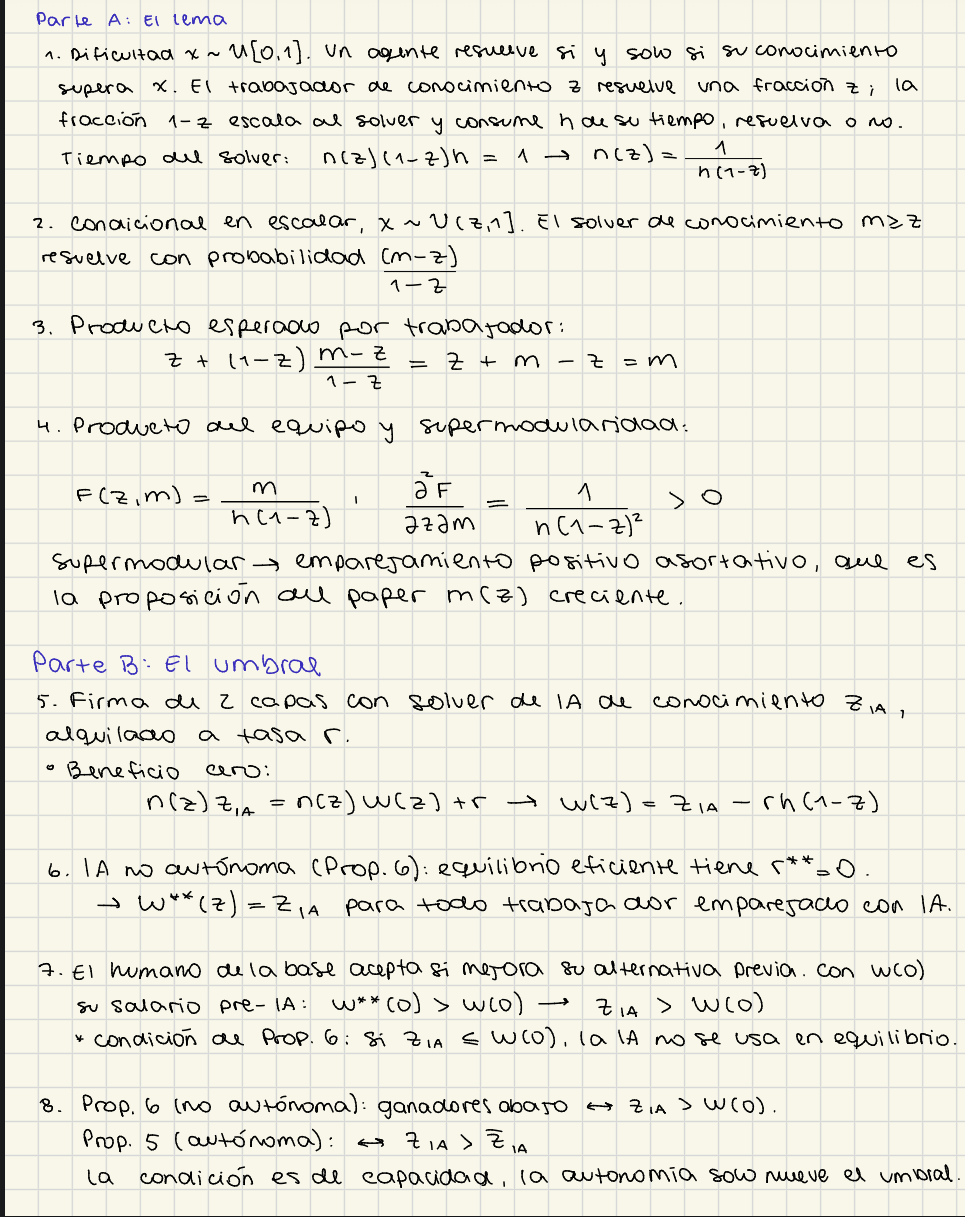
\includegraphics[height=.76\textheight,width=\linewidth,keepaspectratio]{hand/manual-verification.png}
\end{columns}
\sourcefoot{Foto de la estudiante, sin modificaciones. Contraste: §3.1, pp. 9--12; Props. 5--6, pp. 24 y 27.}
\end{frame}

\begin{frame}{Veredicto y alcance de lo aprendido}
\begin{block}{La lectura común es incompleta; su exclusión es falsa}
La autonomía cambia los usos posibles y el costo de oportunidad. La capacidad decide cuándo se cruza cada umbral. Ninguna dimensión sustituye a la otra.
\end{block}
\begin{itemize}
\item $w(0)<\bar a$: hay una franja donde N ayuda a la base y A no le da ganancia estricta frente a no IA.
\item El conflicto A--N cubre todo $a<1$: debajo de $w(0)$, N evita pérdidas aunque no se adopte; encima hay ganancia estricta.
\item SymPy y LP verifican piezas y ejemplos. La prueba general del continuo no se sustituye por una malla.
\item Límites pendientes: ampliar la hoja con el caso discreto, probar el equilibrio en Lean y revisar las fronteras de régimen.
\end{itemize}
\sourcefoot{Props. 5--6, pp. 24--27; comparación y evaluación propias. Ver extensions.md.}
\end{frame}
\end{document}
